\documentclass[10pt,preprint]{sigplanconf}

\usepackage[utf8]{inputenc}
% the following standard packages may be helpful, but are not required
%\usepackage{longtable}
\usepackage{mathtools}
\usepackage{multicol}
\usepackage{multirow}
\usepackage{booktabs}
\usepackage{courier}
\usepackage[scaled]{helvet}
\usepackage{url}
\usepackage{listings}
\usepackage{enumitem}
\usepackage{mdwlist} % tighter description environment (starred)
\usepackage[colorlinks=true,allcolors=blue,breaklinks,draft=false]{hyperref}
% known bug: http://tex.stackexchange.com/questions/1522/pdfendlink-ended-up-in-different-nesting-level-than-pdfstartlink
\newcommand{\doi}[1]{doi:~\href{http://dx.doi.org/#1}{\Hurl{#1}}}   % print a hyperlinked DOI

\usepackage{graphicx}
\usepackage{softdev}
\usepackage{amsmath}
\usepackage{mdwlist}
\usepackage{pifont}

\lstset{
	basicstyle=\tt\scriptsize,
	xleftmargin=2em,
    framexleftmargin=1.5em,
	numberstyle=\scriptsize\tt\color{gray},
	captionpos=b,
	escapeinside={{<!}{!>}},
}

\begin{document}

\title{Virtual Machines in the Cold: Investigating Warmup}
\authorinfo{Edd Barrett}
           {Software Development Team\\ Department of Informatics\\ King's College London}
           {http://eddbarrett.co.uk/}
\authorinfo{Carl Friedrich Bolz}
           {Software Development Team\\ Department of Informatics\\ King's College London}
           {http://cfbolz.de/}
\authorinfo{Laurence Tratt}
           {Software Development Team\\ Department of Informatics\\ King's College London}
           {http://tratt.net/laurie/}

\maketitle

\noindent\textbf{Please note: this is a draft.}

\begin{abstract}
Warmup is magic.
\end{abstract}

\section{Introduction}
\label{sec:intro}

\laurie{we need a really simple graph in the intro, along the lines of the one
in the glowworm proposal. and not the current figure 1, whose caption is really
confusing!}

\laurie{since, at the moment, we don't say anything about how \emph{long} it
takes to warmup, i've not tried saying at all about that.}

Many modern languages are implemented as Virtual Machines (VMs) which use a
Just-In-Time (JIT) compiler to translate programs into machine code at run-time.
Since this compilation is not immediate, programs which are JIT compiled are
said to be subject to a \emph{warmup} phase. During the warmup phase, program
execution is slow; after warmup, execution is fast. Although users new to JIT
compiled VMs are surprised by the effects of warmup, it is a widely understood
phenomenon and shared by all JIT compiled VMs. Typically, benchmarking programs
on JIT compiled VMs involves running a benchmark a number of times, discarding
the first $n$ iterations where the VM is in the warmup phase, and reporting the
result of the remaining iterations.

In this paper, we show that the traditional notion of warmup is not generally
applicable to modern JIT compiled VMs. We present a carefully designed
experiment that allows us to run a number of simple benchmarks on a variety of
VMs for a large number of iterations. We expected this to represent an ideal
situation that would allow us to easily compare warmup across VMs. However, the
results are surprising: some benchmarks on some VMs run as per traditional
expectations; some never warmup at all, staying at their initial performance
levels indefinitely; and some `warmdown', getting slower over time. Even within
those benchmarks that appear to warmup in a traditional fashion, there are
various performance patterns that make presenting a simple performance number
difficult. \laurie{is is true?} Of the \laurie{however many} VMs we looked at,
none consistently warmsup in the traditional notion.

Our results suggest that, as a field, we need to take a more nuanced view
of warmup. In general, we suggest it is better to think of most benchmarks as
generally converging on a \emph{steady state} of performance (be that faster or
slower than initial execution). When a benchmark does not converge on a steady
state, we suggest that it is impossible to give meaningful performance figures.
We believe our results are of interest both to VM writers and users of those
VMs. VM authors may not have previously considered the different possible types
of warmup behaviour, or found small benchmarks which trigger such behaviour.
Users of VMs may obtain greater understanding of why their particular program
does not perform as well on a JIT compiled VM as they expected.

This paper's contributions are as follows:
\begin{enumerate*}
  \item \laurie{blah blah}
\end{enumerate*}

This paper's structure is as follows. \laurie{blah blah}


\section{Conceptions of Warmup}
\label{sec:warmup}

\sarah{This is nice, because it defines the sort of thing that might be important in a model of idealised JIT behaviour.
Steady state implies low latency AND low variance of latency?}
The term ``warmup'' refers to the way in which language runtimes tend to take
time to reach a steady state of peak performance. The term is mostly used when
talking about JIT compilers. A typical VM
with a JIT begins executing a program in a profiling interpreter. Information
gathered through profiling is then used as a heuristic to decide which portions
of the program are good candidates for compilation to fast native code. Once a
candidate has been compiled, the VM uses the fast native code in the future
(instead of the slow interpreter), thus improving performance.  Although
interpretation, profiling and compilation all come with a performance hit,
ideally there should be a point at which the VM has all of the binary code it
needs to execute the whole program natively. At this point, interpretation,
profiling and compilation should no longer occur, and thus peak performance is
met. Between the start of the VM's execution and the point at which peak
performance is met, the JIT is said to be ``warming up''.\edd{graph is in a
different style to the others. If we decide this is a good example, ping me
and I will re-do it}.

\begin{figure}[h!]
\centering
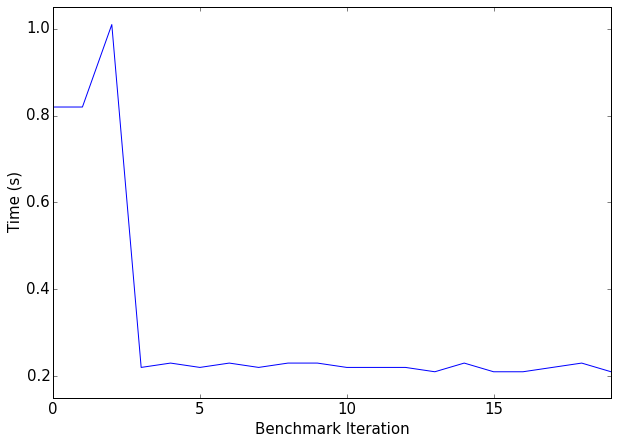
\includegraphics[width=.4\textwidth]{img/trad}
\caption{This (fictional) chart illustrates the commonly accepted understanding
of JIT performance. Early iterations of a benchmark perform poorly during the
warmup phase of the JIT. Once the JIT begins emitting native code (around
iteration 3) the latency of the benchmark is consistently small, with a small
amount of variation due to the operating system and execution environment.}
\label{fig:trad}
\end{figure}

\sarah{If context switches can introduce noise, presumably the measurement of latency here is wall-clock time.
In which case this might be mentioned a little earlier in the paper, to clarify what ``performant'' means in the rest of the paper.}
The graph in Figure~\ref{fig:trad} demonstrates the impact that we might
expect JIT warmup to have upon a benchmark running repeatedly within a
single process. In the first iteration (iteration 0), the VM has no compiled
code for the benchmark and therefore it runs slowly in a profiling
interpreter. After two or three iterations the profiler has collected enough
information for the JIT the begin compiling. For this fictional VM,
compilation is more expensive than the profiling interpreter, thus it is
characterised by the spike at iteration 2. \footnote{The cost of
the profiling interpreter relative to that of compilation vary on a per-VM
basis.}At iteration 3, the JIT has compiled all of the code necessary to
efficiently run the benchmark. Subsequent iterations use the compiled code
and therefore run with improved performance. In other words, peak
performance is achieved at iteration 3. Note however that the measured times
for iterations $\geq 3$ are not quite the same. This is because there are many
sources of random variation that impact benchmark measurements. Random
variation can be introduced by the underlying operating system (e.g. by
context switches), or by the VM itself (e.g. garbage collection).  Generally
speaking, we expect peak performance measurements to be fast and ``mostly
constant'', with only small random variations distributed around a constant
mean~\cite{XXX}.  Ideally it would be possible to identify and control the
sources of random variation, allowing us to measure only the performance
characteristics of the VM. In practice however, this is very difficult.

A handful of methodologies -- most notably
\cite{kalibera12quantifying,kalibera13rigorous} -- require experimenters to take
warmup into account when benchmarking. We therefore set out to quantify how long
it takes various JIT compiled VMs to warmup. However, it soon became apparent to
us that our understanding of warmup is extremely naive:


\section{Benchmarking Methodology}
\label{sec:methodology}

To decide whether expected impact of JIT warmup (as outlined in the previous
section) tallies with reality, we devised an experiment.  The goal of the
experiment is to measure the long-term effects of warmup upon benchmarks,
whilst controlling as many confounding variables as is practically
possible.

We began with a suite of benchmarks, most of which were collected from Laurence
Tratt's VM experiment~\cite{XXX}. Each benchmark is implemented in multiple
languages allowing us to run them on a range of different VMs. The benchmarks
were modified so as to hook into our benchmark runner, \emph{Krun}. Krun has
been designed to
help measure JIT warmup on Linux systems. Specifically Krun attempts to address
random variation introduced by:
%
\begin{description*}
\item[Ambient temperature changes] Benchmarks can heat up the system hardware
potentially impacting performance. Krun measures the temperature of the machine
prior to benchmarking, then before starting each benchmark, it waits for the
system temperature to return to within 10$\%$ hotter than the starting
temperature. All temperature zones are checked, and if the system fails to cool
within a resonable time, Krun terminates.
\item[Processes sharing the same CPU] Other processes running on the same CPU
as benchmarks can impact performance. Krun therefore insists that benchmarks
are run on an isolated CPU core.~\footnote{We use the \texttt{isolcpus} feature
of the Linux kernel to achieve this. This means that benchmarks share a CPU
only with kernel threads. In theory a core can be fully isolated, however the
Linux tool to enable this is currently broken
(\url{https://bugs.debian.org/cgi-bin/bugreport.cgi?bug=796893})}
\item[The \emph{perf} subsystem] By default, Linux has a kernel profiler,
\emph{perf}, running. This is a significant source of random variation,
especially since it dynamically adjusts (lowers) its sample rate if it is found
to spend too much CPU time. Perf cannot be disabled on X86-64, but Krun insists
that the perf sample rate is set to the lowest possible value of one sample per
second.
\item[CPU governors] Krun attempts to fix the CPU frequency to the highest
possible value (short of overclocking). This is achieved by disabling Intel
p-states support in the kernel and setting CPU governor to \texttt{performance}
mode.~\footnote{This is our best attempt at obtaining a constant CPU clock
speed. The Linux kernel documentation states that ``the idea that frequency can
be set to a single frequency is fiction for Intel Core
processors''~\cite{XXX}.}
\item[Unexpected events] Linux has a tendency to emit important information
relating to system performance to the \texttt{dmesg(1)} buffer. Krun monitors
this buffer, and in the event of a change, mails the experimenter a unified
diff. It is up to the experimenter to decide if the message has impacted
performance.
\item[Heap Usage] The amount of heap memory available to a VM can impact
performance. Krun therefore restricts the amount of heap memory available to
the VM.
\end{description*}

\edd{data layout (e.g. ASLR, don't re-run in separate sessions)}
\edd{quartile regression}

We ran the benchmarks on a collection of modern programming language VMs:
\begin{description*}
\item[PyPy-2.6.0] A meta-tracing VM for Python-2.7.
\item[Java8-b132] Oracle's Hotspot VM for Java.
\item[Graal-dev~\footnote{Graal version 9dafd1dc5ff9.}] Oracle's next-gen
Java VM.
\item[LuaJIT-2.0.4] A tracing JIT for Lua.
\item[HHVM] Facebook's PHP JIT.
\item[JRuby/Truffle-dev~\footnote{JRuby/Truffle version 7b4cee81891f.}] A
Ruby VM using Graal/Truffle.
\item[V8-4.5.38] Google's JIT for Javascript.
\item[CPython-2.7.10] The reference Python implementation.
\end{description*}

All bar one of
these VMs include a JIT compiler. CPython is a simple interpreter written in C,
that was included as a kind of sanity check (it should not exhibit JIT warmup
characteristics). We ran the following benchmarks:

\begin{description*}
\item[binarytrees] Allocates, walks and deallocates binary trees.
\item[richards] Simulates an operating system's task scheduler.
\item[spectralnorm] Computes the spectral norm of a matrix.
\item[nbody] Models the orbits of planets.
\item[fasta] Performs various computations on DNA sequences.
\item[fannkuch] Mutates a sequence of integers until a fix-point.
\end{description*}


We ran each benchmark with 2000 in-process iterations,
and repeated this twice for each benchmarking machine involved. We used two
similar X86-64 machines: the first a quad-core i7-4790K running at 4GHz with
an 8MB cache and 24GB of RAM; the second, an Intel i7-4790 running at 3.6GHz
with 8MB of cache and 32GB of RAM. Both machines run Debian 8 and have Intel
Turbo Boost disabled in the BIOS. All VMs were restricted to using at most
2GB of heap. We did \emph{not} force garbage collection after each
in-process iteration of a benchmark \cfbolz{we need to argue why we don't do anything special about GC}

\section{Results}
\label{sec:Results}

After running all benchmarks as described we analysed the benchmarks in a
two-step process. In the first step we visually inspected the run sequence
graphs of all the benchmark executions, per benchmark and virtual machine. In
doing so we noted whether the virtual machine followed the expected warmup
behaviour for this benchmark as described in Section~\ref{sec:warmup}. This was
the case of \cfbolz{add numbers} X out of Y benchmarks. In a second step we
identified groups of ``anomalies'', i.e. repeating ways of how benchmark
executions deviated from the expected warmup behaviour. In the following we will
present the run-sequence diagrams of benchmarks that have expected warmup
behaviour, as well descriptions and examples for all the anomalies.

\cfbolz{need some examples of nice benchs}
\cfbolz{we need a table which does all the categorizations, and examples}

\cfbolz{observations 2x2: widely varying performance on the same machine, late
phase change not always there, another case: bimodality, slowdowns are
sometimes speedups, different repeating shapes across machines}

\cfbolz{safety checks: are outliers deterministic across different processes?
is the behaviour generally the same looking? do some checks on other OS,
machine architecture, frequency scaling independent}


\sarah{Warm-up takes longer than expected, by comparison with the idealised JIT
described in Section 2.}


\subsection{Outliers}
\label{sub:outliers}

Outliers are iterations of a benchmark that take significantly longer than the
other iterations, even taking the randomness of the benchmark iterations into
account.

Figure~\ref{fig:examples:outliers1} shows one such example.

\begin{figure}[h!]
\centering
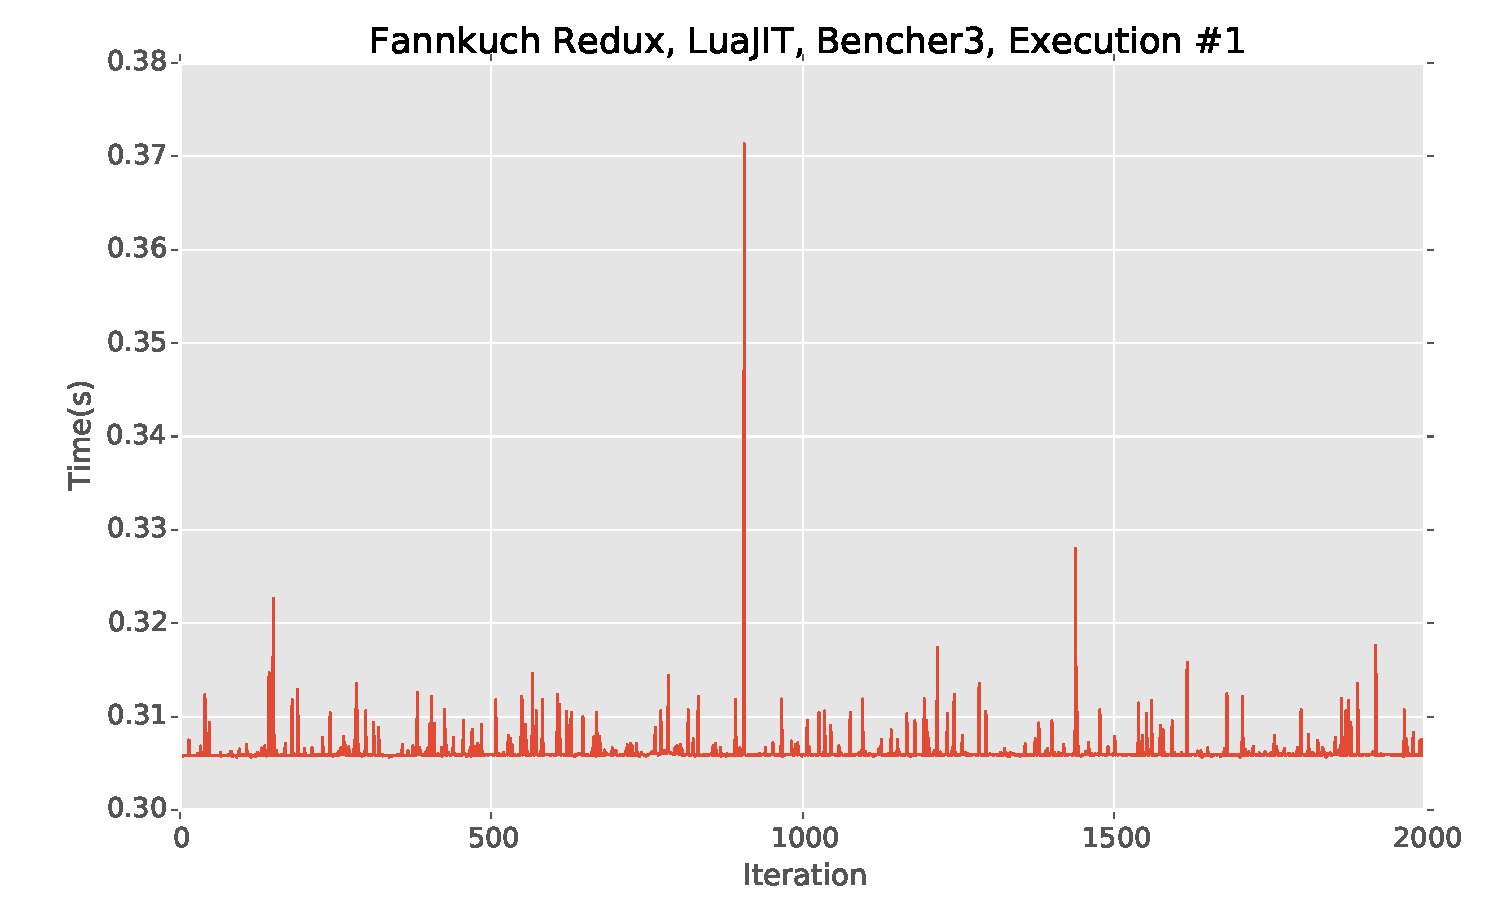
\includegraphics[width=.46\textwidth]{examples/outliers1}
\caption{Example of a benchmark with outliers.}
\label{fig:examples:outliers1}
\end{figure}


\subsection{Slowdowns}
\label{sub:slowdowns}

\sarah{This is one area were the sliding-window average might be useful (i.e. in detecting a slow-down).
One possible way forward would be to find a technique for performing hypothesis testing on time-series data, then running tests to determine whether the sliding-mean in one part of the chart is significantly different to the sliding-mean in an earlier phase of the execution.
This technique would also help to determine precisely when the warm-up phase is over and the JIT has kicked in.}

A few benchmarks exhibit slow downs, where the first few iterations of a
benchmarks are faster than the eventual mean after ``warm up''.

Figure~\ref{fig:examples:slowdown1} shows one such example.

\begin{figure}[h!]
\centering
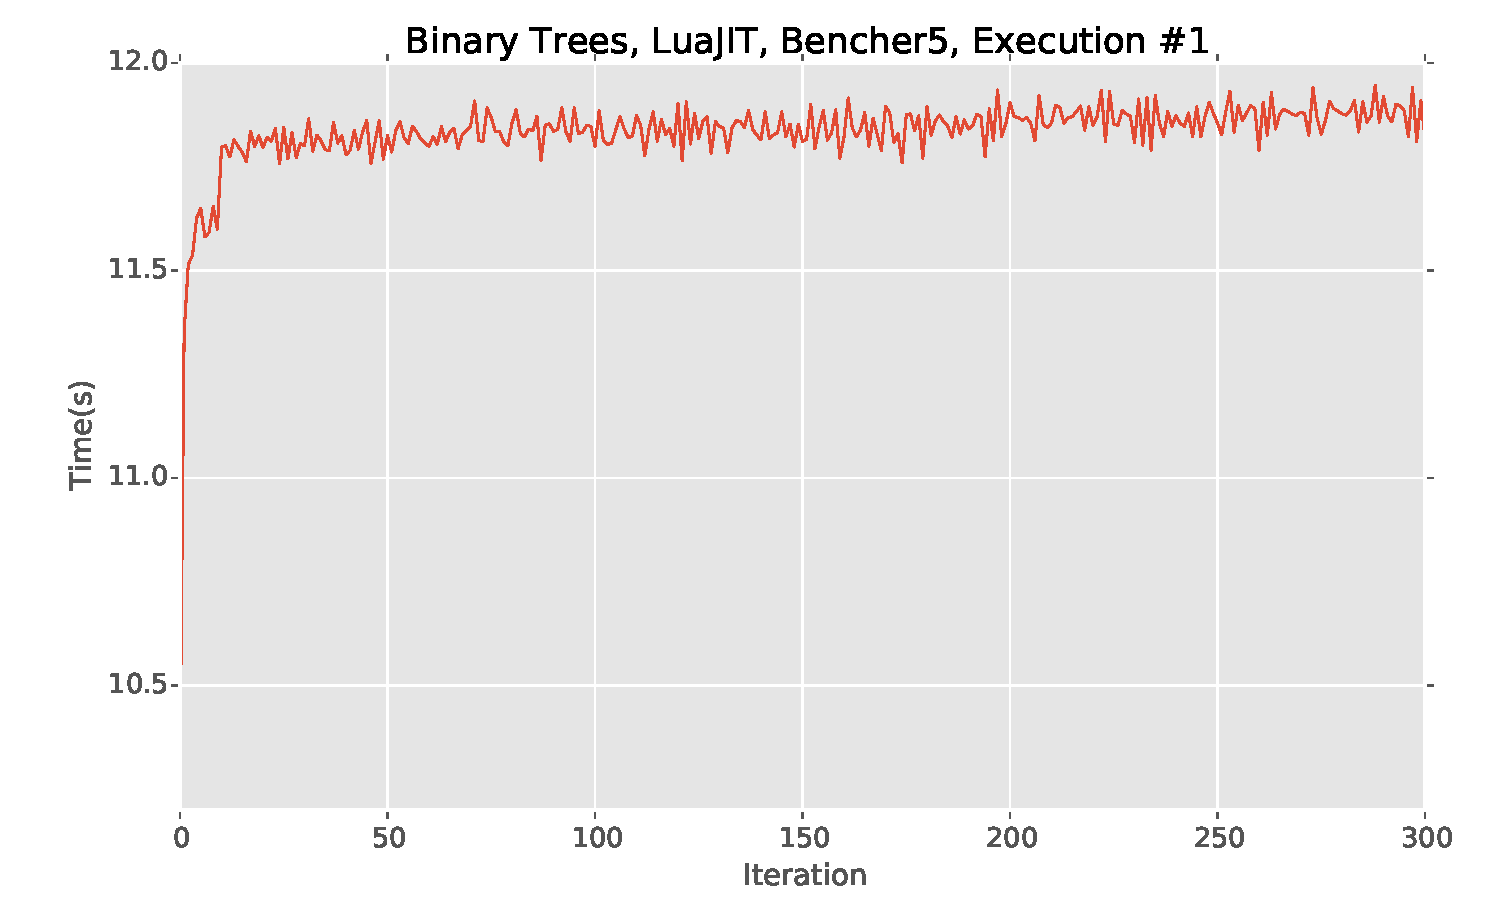
\includegraphics[width=.46\textwidth]{examples/slowdown1}
\caption{Example of a benchmark with a slowdown.}
\label{fig:examples:slowdown1}
\end{figure}



\subsection{Cyclic Behaviour}
\label{sub:cyclic}

Cyclic behaviour occurs in a number of benchmarks, which is a pattern of $n$
iterations that have similar timing results and keeps repeating across the
benchmark runs.

Figure~\ref{fig:examples:cycles1} shows one such example.

\begin{figure}[h!]
\centering
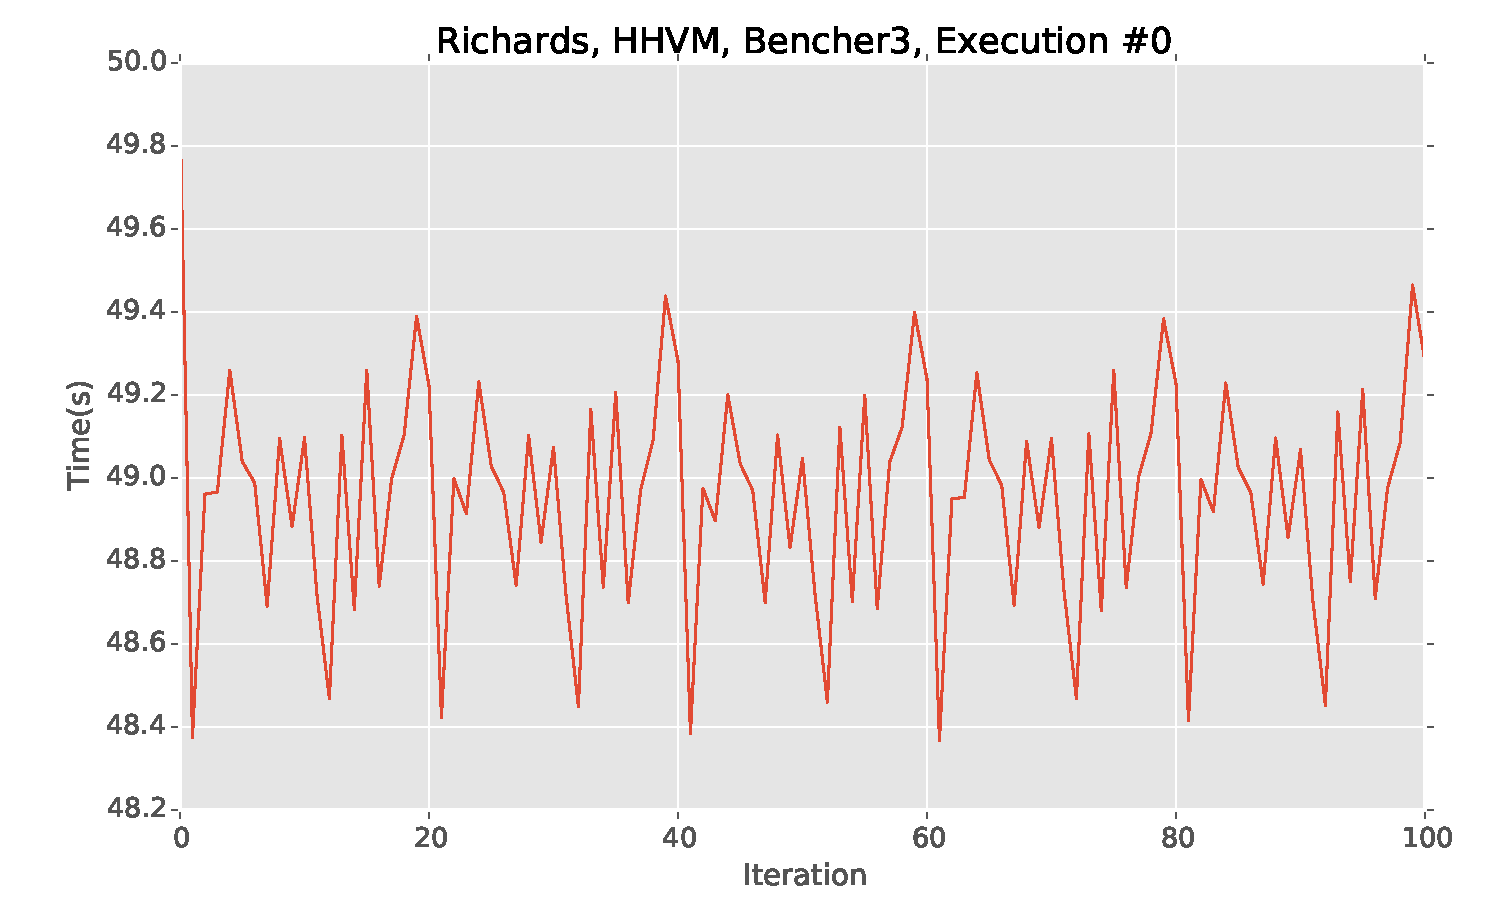
\includegraphics[width=.46\textwidth]{examples/cycles1}
\caption{Example of a benchmark with cycles.}
\label{fig:examples:cycles1}
\end{figure}


\subsection{Late Phase Changes}
\label{sub:phase}

Late phase changes occur in benchmarks where after many iterations the benchmark
changes behaviour, either by getting slower or faster, or by producing a
different pattern of randomness.

Figure~\ref{fig:examples:late1} shows one such example.

\begin{figure}[h!]
\centering
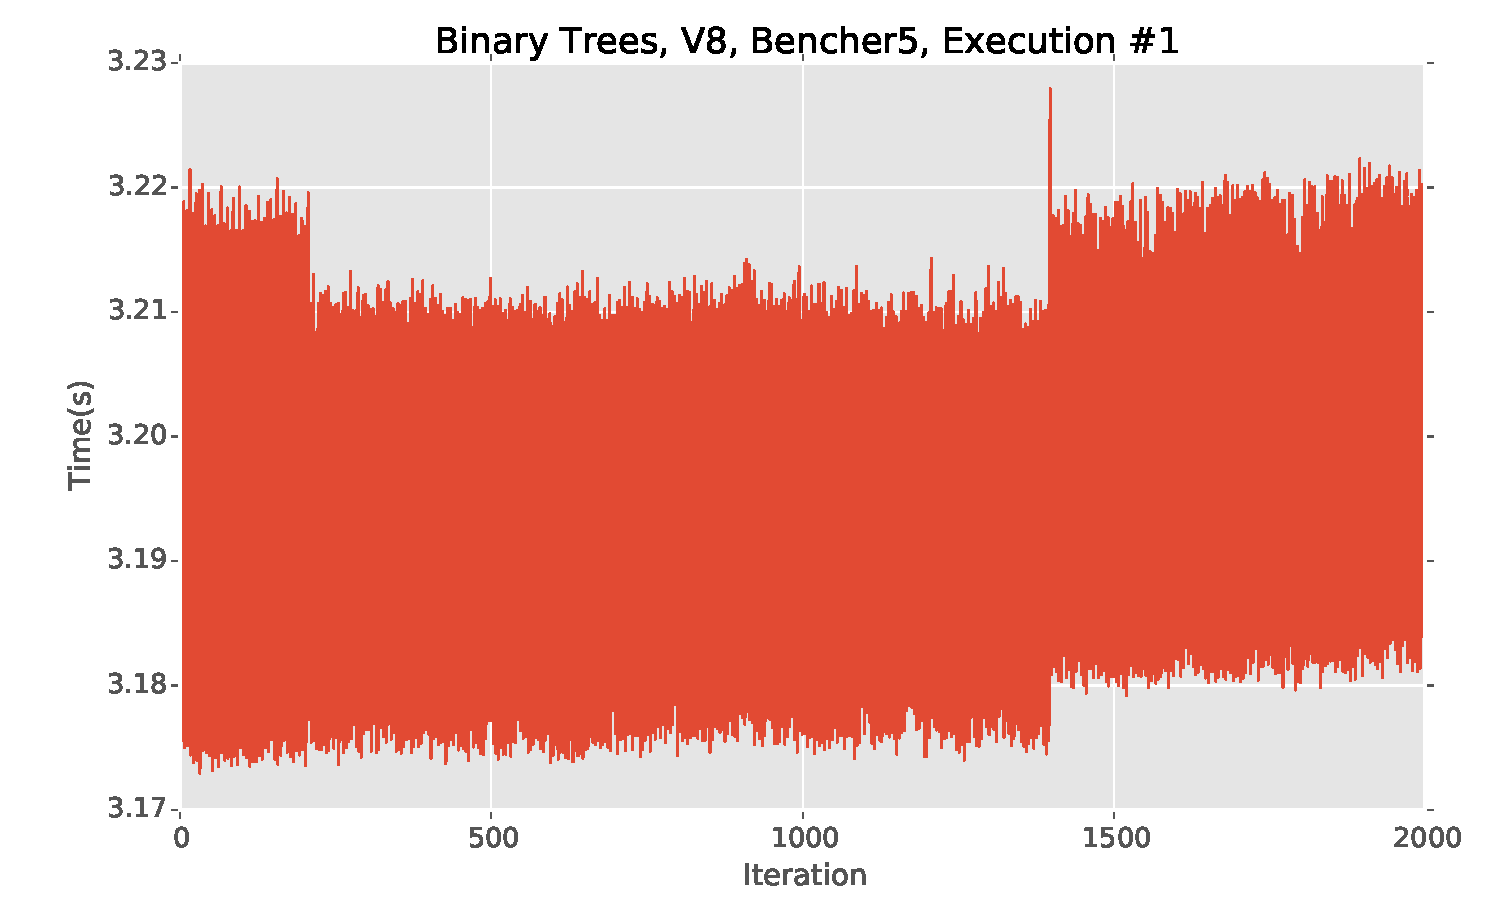
\includegraphics[width=.46\textwidth]{examples/late1}
\caption{Example of a benchmark with late phase changes.}
\label{fig:examples:late1}
\end{figure}

\subsection{Inconsistent Effects}
\label{sub:inconsistent}

\edd{Many of the effects we saw are consistently weird. Some are not. What
do we think of this as a section?}

Figure~\ref{fig:examples:consistent_weirdness1} shows a case where
unexpected behaviours are consistent between machines and executions.
Figure~\label{fig:examples:inconsistent_weirdness1} shows an example where
effects differ between both machines and executions.

\begin{figure*}[h!]
\centering
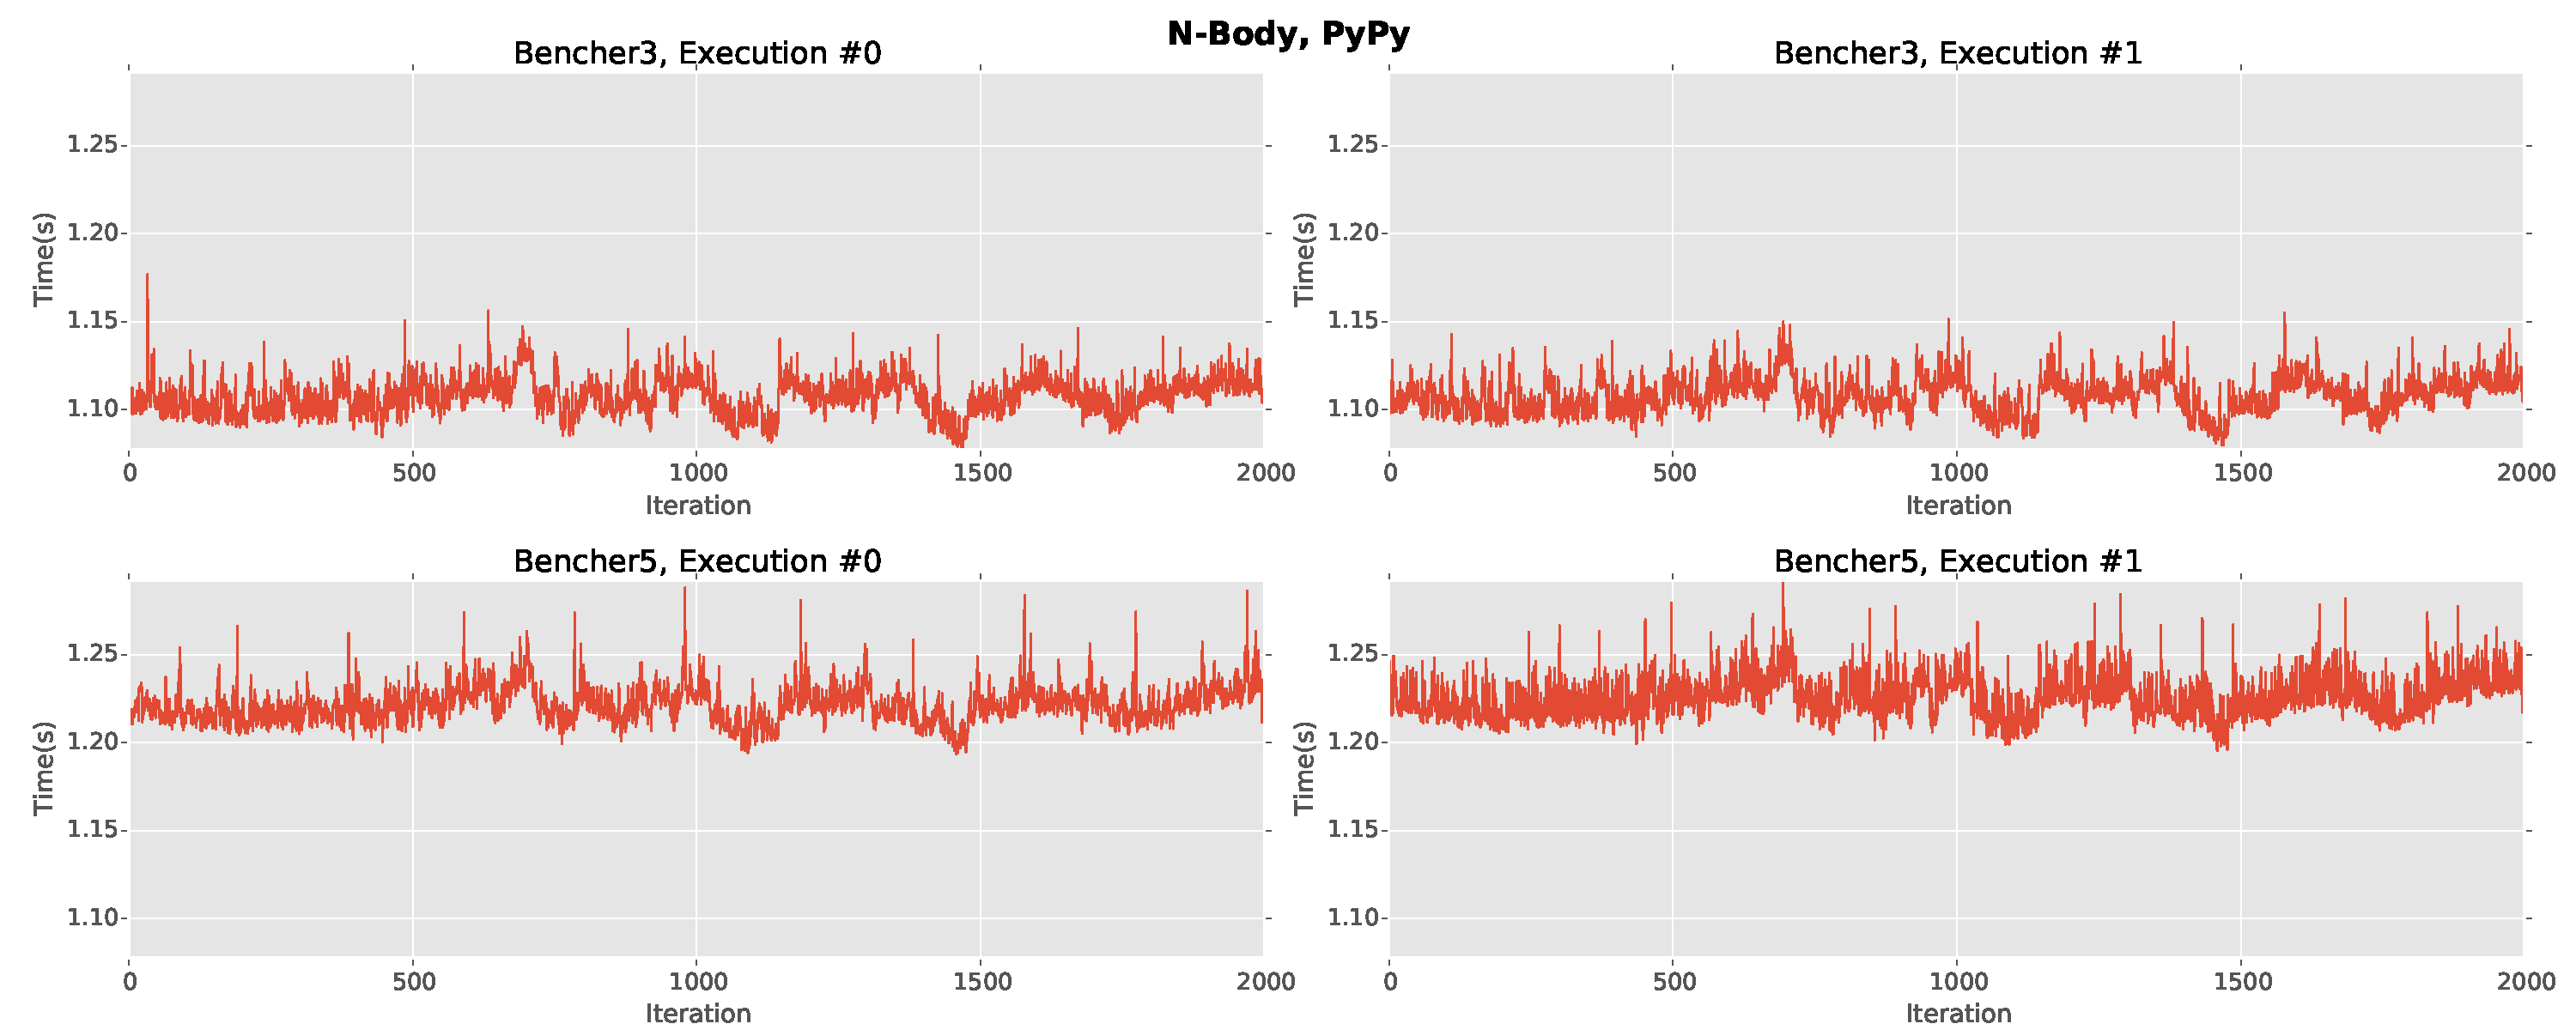
\includegraphics[width=\textwidth]{examples/consistent_weirdness1}
\caption{Example of a benchmark whose effects are consistent between machines and executions.}
\label{fig:examples:consistent_weirdness1}
\end{figure*}

\begin{figure*}[h!]
\centering
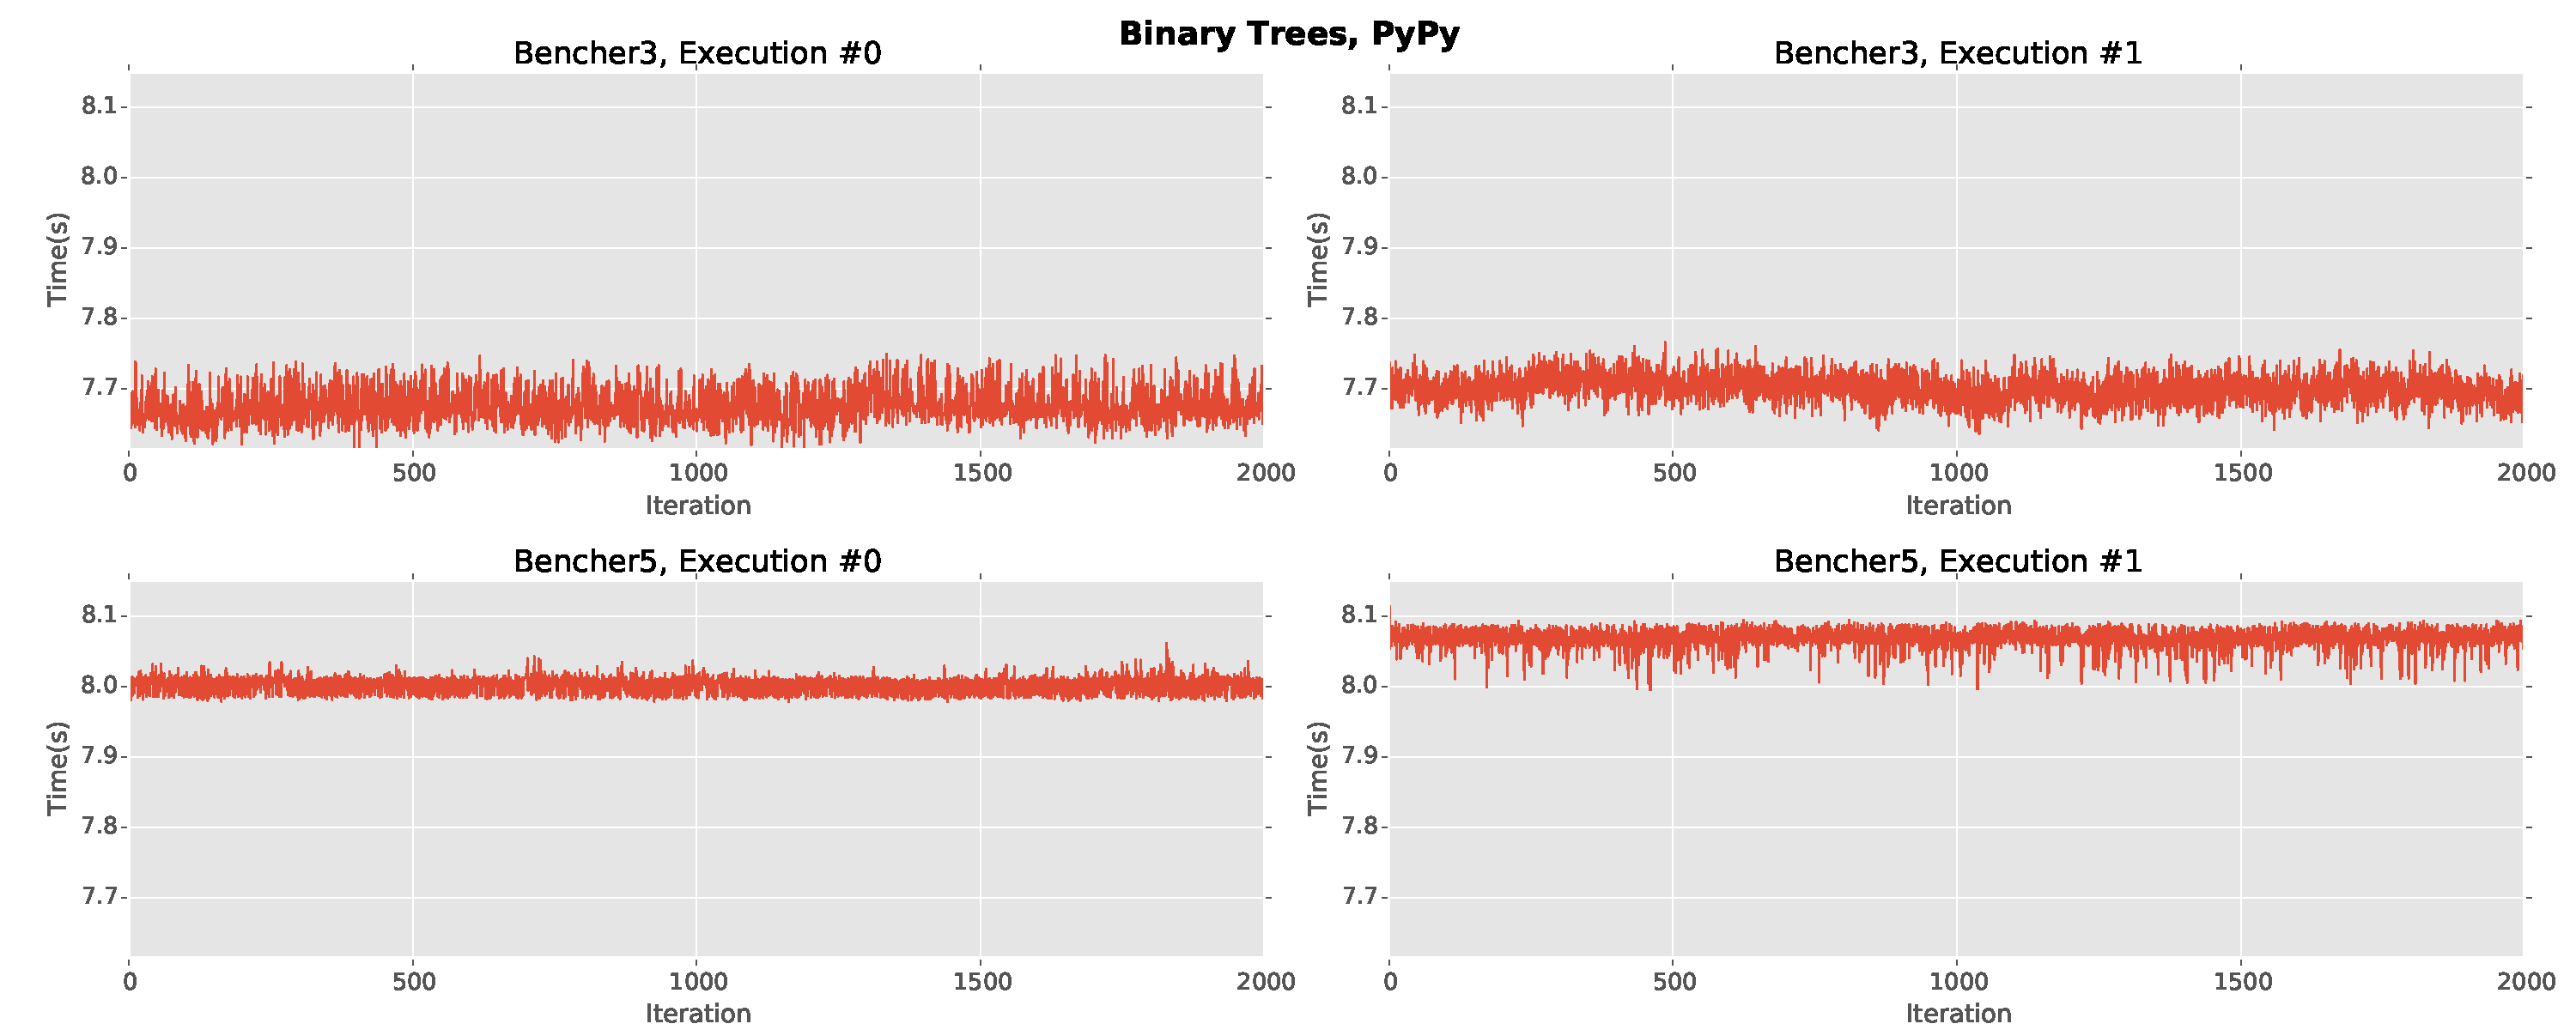
\includegraphics[width=\textwidth]{examples/inconsistent_weirdness1}
\caption{Example of a benchmark whose effects are inconsistent between machines and executions.}
\label{fig:examples:inconsistent_weirdness1}
\end{figure*}

\section{Threats to Validity}
\label{sec:threats}

\sarah{threats to validity: there may be some confounding variables that have
not been controlled in these experiments. There may be bugs in the JITs that
are being measured.  The benchmarks in the guest languages might be similar
enough that some important classes of behaviour have been missed, because the
benchmarks here do not trigger those behaviours.  There may be some un-thought
of explanation for weird JIT behaviour which has nothing to do with the JIT.}


\section{Discussion}
\label{sec:Discussion}

  - discussion:
    - need to give up naive definition of warmup
    - unrealistic to get rid of these anomalies
    - some of benchmarking wisdom is wrong in the presence of this stuff
\sarah{Need some way to model the behaviour of JITs and perform hypothesis tests (so that people can answer questions like 'does this change in the VM actually make the JIT faster?').}

\section{Conclusions}
\label{sec:conclusion}

\bibliographystyle{abbrvnat}
\bibliography{bib}


\end{document}

